\documentclass[10pt,a4paper,notitlepage]{article}
\usepackage[utf8]{inputenc}
\usepackage[french]{babel}
\usepackage[T1]{fontenc}
\usepackage{mathtools}
\usepackage[left=2cm,right=2cm,top=2cm,bottom=2cm]{geometry}
\usepackage{graphicx}
\usepackage{float}
\usepackage{subcaption}
\usepackage{tikz}

\addto{\captionsfrench}{\renewcommand{\abstractname}{Introduction}}

\author{Pierre-Antoine Comby}
\title{TP1 : Commande d'un bras à liaison flexible par bouclage linéarisant}

\usepackage{enumitem}
\setlist[itemize]{label=\textbullet}

%ensembles usuels
\newcommand{\R}{\mathbb{R}}
\newcommand{\C}{\mathbb{C}}
\newcommand{\N}{\mathbb{N}}
\newcommand{\Z}{\mathbb{Z}}

\newcommand{\K}{\mathbb{K}}
\newcommand{\M}{\mathcal{M}}
\newcommand{\Lin}{\mathcal{L}}
\newcommand{\Img}{\text{Im}}
\newcommand{\Ker}{\text{Ker}}
\newcommand{\A}{\text{A}}
\newcommand{\B}{\text{B}}
\newcommand{\fromatob}{\A\to\B}

\DeclareFontFamily{U}{wncy}{}
\DeclareFontShape{U}{wncy}{m}{n}{<->wncyr10}{}
\DeclareSymbolFont{mcy}{U}{wncy}{m}{n}
\DeclareMathSymbol{\Sh}{\mathord}{mcy}{"58}

%relations

\newcommand{\eqv}{\Leftrightarrow}
\newcommand{\tr}{{}^t\! }

\DeclareMathOperator*{\equals}{=}

\newcommand{\limfty}[1]{\xrightarrow[#1 \to +\infty]{}}
\newcommand{\simfty}{\underset{+\infty}{\sim}}

\newcommand{\intinfty}{\int_{-\infty}^{+\infty}}

\renewcommand{\d}{\mathrm{d}}
\newcommand{\dd}[2]{\frac{\d #1}{\d #2}}
\newcommand{\ddd}[2]{\frac{\d^2 #1}{\d {#2}^2}}
\newcommand{\dr}[2]{\frac{\partial #1}{\partial #2}}
\newcommand{\divv}{\text{div}}
\newcommand{\grad}{\text{grad}}
\newcommand{\et}{\quad\text{ et }\quad}
\newcommand{\avec}{\quad\text{ avec }\quad}
\newcommand{\sinon}{\quad\text{ sinon }\quad}
\newcommand{\skzi}{\sum_{k=-\infty}^{+\infty}}
%Macros mieux :)
\newcommand{\chimie}[1]{$\mathrm{#1}$}
\newcommand{\chimiecite}[1]{\[\mathrm{#1}\]}
\newcommand{\nchim}{\mathit{n}}
\newcommand{\xchim}{\mathit{x}}
\renewcommand{\unit}[1]{~\mathrm{#1}}
\renewcommand{\d}{\mbox{d}}
\newcommand{\deriv}[2][]{\frac{\d#1}{\d#2}}
\newcommand{\derivp}[2][]{\frac{\partial#1}{\partial#2}}
\newcommand{\derivpp}[2][]{\frac{\partial^2#1}{\partial#2^2}}

\newcommand{\NA}{\mathcal{N}_A}% Avogadro
\newcommand{\e}{\text{e}}
\newcommand{\sinc}{\text{sinc}}

\newcommand{\fonct}[4]{%
\left\lbrace \begin{array}{l}
{#1}\longrightarrow {#2} \\
{#3}\longmapsto {#4}
\end{array}\right.}
\newcommand{\vect}[1]{%
  \begin{bmatrix}
    #1
  \end{bmatrix}
}

\makeatletter

\@ifpackageloaded{circuitikz}{%
\tikzset{every picture/.style={execute at begin picture={%
   \shorthandoff{:;!?};}}}}{}

\@ifpackageloaded{stmaryrd}{%
\newcommand{\entint}[1]{\llbracket #1 \rrbracket}}{}
\@ifpackageloaded{siunitx}{%
%\newcommand{\gdr}[3]{\ensuremath{#1 = }\SI{#2}{#3}}

}{}
\@ifpackageloaded{listings}{%
\usepackage{xcolor}

\AtBeginDocument{%
\lstset{
    language=Python,
    basicstyle=\ttfamily\small,
    aboveskip={1.0\baselineskip},
    belowskip={1.0\baselineskip},
    columns=fixed,
    extendedchars=true,
    breaklines=true,
    tabsize=4,
    prebreak=\raisebox{0ex}[0ex][0ex]{\ensuremath{\hookleftarrow}},
    frame=lines,
    showtabs=false,
    showspaces=false,
    showstringspaces=false,
    keywordstyle=\color[rgb]{0.627,0.126,0.941},
    commentstyle=\color[rgb]{0.133,0.545,0.133},
    stringstyle=\color[rgb]{01,0,0},
    numbers=left,
    numberstyle=\small,
    stepnumber=1,
    numbersep=10pt,
    captionpos=t,
    literate={{á}{{\'a}}1 {é}{{\'e}}1 {í}{{\'i}}1 {ó}{{\'o}}1 {ú}{{\'u}}1
  {Á}{{\'A}}1 {É}{{\'E}}1 {Í}{{\'I}}1 {Ó}{{\'O}}1 {Ú}{{\'U}}1
  {à}{{\`a}}1 {è}{{\`e}}1 {ì}{{\`i}}1 {ò}{{\`o}}1 {ù}{{\`u}}1
  {À}{{\`A}}1 {È}{{\'E}}1 {Ì}{{\`I}}1 {Ò}{{\`O}}1 {Ù}{{\`U}}1
  {ä}{{\"a}}1 {ë}{{\"e}}1 {ï}{{\"i}}1 {ö}{{\"o}}1 {ü}{{\"u}}1
  {Ä}{{\"A}}1 {Ë}{{\"E}}1 {Ï}{{\"I}}1 {Ö}{{\"O}}1 {Ü}{{\"U}}1
  {â}{{\^a}}1 {ê}{{\^e}}1 {î}{{\^i}}1 {ô}{{\^o}}1 {û}{{\^u}}1
  {Â}{{\^A}}1 {Ê}{{\^E}}1 {Î}{{\^I}}1 {Ô}{{\^O}}1 {Û}{{\^U}}1
  {œ}{{\oe}}1 {Œ}{{\OE}}1 {æ}{{\ae}}1 {Æ}{{\AE}}1 {ß}{{\ss}}1
  {ű}{{\H{u}}}1 {Ű}{{\H{U}}}1 {ő}{{\H{o}}}1 {Ő}{{\H{O}}}1
  {ç}{{\c c}}1 {Ç}{{\c C}}1 {ø}{{\o}}1 {å}{{\r a}}1 {Å}{{\r A}}1
  {€}{{\euro}}1 {£}{{\pounds}}1 {«}{{\guillemotleft}}1
  {»}{{\guillemotright}}1 {ñ}{{\~n}}1 {Ñ}{{\~N}}1 {¿}{{?`}}1}
}
\lstset{language=Matlab,%
    %basicstyle=\color{red},
    breaklines=true,%
    morekeywords={matlab2tikz},
    keywordstyle=\color{blue},%
    morekeywords=[2]{1}, keywordstyle=[2]{\color{black}},
    identifierstyle=\color{black},%
    stringstyle=\color{mylilas},
    commentstyle=\color{mygreen},%
    showstringspaces=false,%without this there will be a symbol in the places where there is a space
    numbers=left,%
    numberstyle={\tiny \color{black}},% size of the numbers
    numbersep=9pt, % this defines how far the numbers are from the text
    emph=[1]{for,end,break},emphstyle=[1]\color{red}, %some words to emphasise
    literate=
    {á}{{\'a}}1 {é}{{\'e}}1 {í}{{\'i}}1 {ó}{{\'o}}1 {ú}{{\'u}}1
    {Á}{{\'A}}1 {É}{{\'E}}1 {Í}{{\'I}}1 {Ó}{{\'O}}1 {Ú}{{\'U}}1
    {à}{{\`a}}1 {è}{{\`e}}1 {ì}{{\`i}}1 {ò}{{\`o}}1 {ù}{{\`u}}1
    {À}{{\`A}}1 {È}{{\'E}}1 {Ì}{{\`I}}1 {Ò}{{\`O}}1 {Ù}{{\`U}}1
    {ä}{{\"a}}1 {ë}{{\"e}}1 {ï}{{\"i}}1 {ö}{{\"o}}1 {ü}{{\"u}}1
    {Ä}{{\"A}}1 {Ë}{{\"E}}1 {Ï}{{\"I}}1 {Ö}{{\"O}}1 {Ü}{{\"U}}1
    {â}{{\^a}}1 {ê}{{\^e}}1 {î}{{\^i}}1 {ô}{{\^o}}1 {û}{{\^u}}1
    {Â}{{\^A}}1 {Ê}{{\^E}}1 {Î}{{\^I}}1 {Ô}{{\^O}}1 {Û}{{\^U}}1
    {œ}{{\oe}}1 {Œ}{{\OE}}1 {æ}{{\ae}}1 {Æ}{{\AE}}1 {ß}{{\ss}}1
    {ű}{{\H{u}}}1 {Ű}{{\H{U}}}1 {ő}{{\H{o}}}1 {Ő}{{\H{O}}}1
    {ç}{{\c c}}1 {Ç}{{\\cite{}  C}}1 {ø}{{\o}}1 {å}{{\r a}}1 {Å}{{\r A}}1
    {€}{{\euro}}1 {£}{{\pounds}}1 {«}{{\guillemotleft}}1
    {»}{{\guillemotright}}1 {ñ}{{\~n}}1 {Ñ}{{\~N}}1 {¿}{{?`}}1
  }
}}{}
\makeatother

\renewcommand{\R}{\mathbb{R}}
\renewcommand{\Z}{\mathbb{Z}}
\renewcommand{\vec}{\overrightarrow}
\begin{document}
\maketitle
\section{Modélisation}
\begin{figure}[ht]
  \centering
  \begin{subfigure}{0.5\linewidth}
  \begin{tikzpicture}
    \node[draw,circle] (O) at (0,-2) {};
    \node[draw,circle] (A) at (-3,0) {};
    \node[draw,circle] (B) at (3,0) {};
    \node[draw,circle] (P) at (0,5) {};
    \draw[very thick] (O) -- (P) node[midway,right]{R} (A)--(P)node[midway,left]{$L_1$} (B)--(P)node[midway,right]{$L_2$};
    \draw[latex-latex] (O) -- ++(3,0) node[midway,above]{$r$};
    \draw[latex-latex] (B) -- ++(0,-2) node[midway,right]{$d$};
  \end{tikzpicture}
  \subcaption{Bras en position stationnaire}
\end{subfigure}%
  \begin{subfigure}{0.5\linewidth}
  \begin{tikzpicture}
    \node[draw,circle] (O) at (0,-2) {};
    \node[draw,circle] (A) at (-3,0) {};
    \node[draw,circle] (B) at (3,0) {};
    \node[draw,circle] (P) at (-1,5) {};
    \node[below=0.7em] at (O) {O};
    \node[left=0.7em] at (P) {P};
    \draw[very thick] (O) -- (P) node[midway,right]{R} (A)--(P)node[midway,left]{$L_1$} (B)--(P)node[midway,right]{$L_2$};
    \draw[latex-latex] (O) -- ++(3,0) node[midway,above]{$r$};
    \draw[latex-latex] (B) -- ++(0,-2) node[midway,right]{$d$};
    \draw[dashed,latex-latex] (B) -- ++(0,5) node[midway,right]{$L_{2y}=L_{1y}$};
    \draw[dashed,latex-latex] (P) -- ++(4,0) node[midway,above]{$L_{2x}$};
    \draw[dashed,latex-latex] (A) -- ++(2,0) node[midway,below]{$L_{1x}$};
    \draw [dashed] (A) ++(2,0) -- (P);
    \draw[dashed] (O) -- ++(0,2.2);
    \draw (O)++(0,2) arc(90:98:2)node[midway,above]{$\psi$};
    \draw (B) ++ (0,1) arc (90:130:1) node[midway,above]{$\theta_2$};
    \draw (P) ++ (0,-1) arc (-90:-113:1) node[midway,below]{$\theta_1$};

  \end{tikzpicture}
  \subcaption{Bras en mouvement}
\end{subfigure}
\caption{Schéma cinématique du système}
\label{fig:label}

\end{figure}

\paragraph{Prépa.1}
À partir de la figure on a :
\begin{align*}
  L_{1x} &= r - \sin(\psi)R \\
  L_{2x} &= r + \sin(\psi)R \\
  L_{1y} &= R\cos(\psi) - d
\end{align*}

\paragraph{Prépa.2} On a par définition:
\begin{align*}
  F_1 &= -k (L_1-L)
  F_2 &= -k (L_2-L)
\end{align*}
On introduit les angles $\theta_1$ et $\theta_2$ tel que :
 \[
   \tan(\theta_1)  =\frac{L_{1x}}{L_{1y}} \text{ et } \tan(\theta_2) =\frac{L_{2x}}{L_{2y}}
 \]
 Alors on a  pour $F_1$ :
 \begin{align*}
   F_{1y} = F_1 \cos(\theta_1) &= F_1 \frac{1}{\sqrt{1+\tan^2(\theta_1)}}\\
                          &= F_1 \frac{1}{\sqrt{1+\left(\frac{L_{1x}}{L_{2y}}\right)^2}} \\
                          &= k\left(\sqrt{L_{1x}^2+L_{1y}^2}-L\right) \frac{L_{1y}}{\sqrt{L_{1y}^2+L_{1x}^2}}\\
                          &= k L_{1y} \left(1- \frac{L}{\sqrt{L_{1y}^2+L_{1x}^2}}\right)
 \end{align*}
 et :
 \begin{align*}
   F_{1x} &= F_1 \sin(\theta_1)\\
          &= F_1 \cos(\theta_1)\tan(\theta_1) \\
          &= k L_{1y} \left(1- \frac{L}{\sqrt{L_{1y}^2+L_{1x}^2}}\right) \frac{L_{1x}}{L_{1y}} \\
          &= k L_{1x} \left(1- \frac{L}{\sqrt{L_{1y}^2+L_{1x}^2}}\right)
 \end{align*}

 On a les mêmes relations pour $F_2$ soit:
 \[
   F_{2x} = k L_{2x} \left(1- \frac{L}{\sqrt{L_{2y}^2+L_{2x}^2}}\right) \text{ et }
   F_{2y} = k L_{2y} \left(1- \frac{L}{\sqrt{L_{2y}^2+L_{2x}^2}}\right)
 \]
 Et alors :
 \[
\vec{F_1} = \vect{-F_{1x} \\-F_{1y}} \text{ et } \vec{F_2} = \vect{F_{2x}\\-F_{2y}}
 \]
 \paragraph{Prépa.3}
 À partir des expression cartésiennes des forces on a le moment :
 \[
   \vec{\mathcal{M}_{0}}(\vec{F}) =\vec{OP}\wedge (\vec{F_1} + \vec{F_2})=
   \vect{R\sin\psi \\ R\cos\psi \\0} \wedge \vect{F_{2x}-F_{1x}\\ F_{2y}-F_{1y}\\0} = M \vec{u_z}
 \]
 Soit :
 \[
   M = R\cos\psi(F_{2x}-F_{1x}) -R\sin\psi(F_{2y}-F_{1y})
 \]
\paragraph{Prépa.4}
On a :
\[
  F_{2x}-F_{1x} = 2kR\sin\psi + krL \left(
   \underbracket{ \frac{1}{\sqrt{L_{2y}^2+L_{2x}^2}}- \frac{1}{\sqrt{L_{1y}^2+L_{1x}^2}}}_{\Delta}
  \right)
  - k\sin\psi RL \left(\underbracket{
    \frac{1}{\sqrt{L_{2y}^2+L_{2x}^2}} + \frac{1}{\sqrt{L_{1y}^2+L_{1x}^2}}
}_{\Sigma}  \right)
\]
En effectuant à l'orde 1 sur $\Sigma$ et $\Delta$ on a:
\[
  \Delta = \frac{r\psi R}{((R-d)^2+r^2)^{3/2}} \text{ et } \Sigma = \frac{2}{\sqrt{(R-d)^2+r^2}}
\]
soit :
\[
  F_{2x}-F_{1x} \simeq 2 k R \psi +  \psi \frac{kr^2RL }{((R-d)^2+r^2)^{3/2}}- 2k\psi RL \frac{1}{\sqrt{(R-d)^2+r^2}} = \psi K_x
\]
Avec
\[
  K_x = 2kR + \frac{kr^2RL}{((R-d)^2+r^2)^{3/2}} -\frac{2kRL}{\sqrt{(R-d)^2+r^2}}
\]

On fait de même pour $F_{2y}-F_{1y}$ soit :
\[
  F_{2y}-F_{1y} = kR(\cos\psi-d)L \Delta = \frac{kR^2(1-d)Lr}{((R-d)^2+r^2)^{3/2}}\psi =K_y \psi
\]

enfin :
\[
  M = RK_x\psi + RK_y\psi^2
\]
Au premier ordre on a :
\[
  M = \underbracket{R \left(2kR + \frac{kr^2RL}{((R-d)^2+r^2)^{3/2}} -\frac{2kRL}{\sqrt{(R-d)^2+r^2}}\right)}_{K_s} \psi
\]
\paragraph{Prépa.5}
Pour le système \{plateforme + bras\} on a l'énergie cinétique:
\[
  E_c= \frac{1}{2}(J_b+J_p)\dot{\alpha}^2+ \frac{1}{2}\dot{\psi}^2
\]

\paragraph{Prépa.6}
Avec l'ensemble de la masse regroupé à son centre de gravité on a a : l'énergie potentielle de \{plateforme + bras\} suivante :
\[
E_p = mgh\cos(\alpha+\psi)
\]
\paragraph{Prépa.7}
On rappel l'expression générale des equations d'Euler-Lagrange:
\[
  \deriv{t}\derivp[E_c]{\dot{q_i}}-\derivp[E_c]{q_i} =Q_i
\]
Avec $q_i $ coordonnée généralisée et $Q_i$ la forcé généralisé associée à $q_i$( qui regroupe energie potentielle dérivée suivant $q_i$ et  les forces s'exercant au système)
On choisit $\alpha$ et $\psi$ comme coordonnée généralisée (système à deux degrès de liberté). Le système est commandé par la MCC, qui exerce un couple $N\phi i$:
\[
  \begin{cases}
    J_b(\ddot{\alpha}+\ddot{\psi})+K_s\psi- mgh \sin(\alpha+\psi) &= 0 \\
    J_b(\ddot{\alpha} + \ddot{\psi})+J_p\ddot{\alpha} -mgh\sin(\alpha+\psi)  &= N\phi i
  \end{cases}
\]
\paragraph{Prépa.8}
À partir de l'équation électrique :
\[
  u =Ri + L \deriv[i]{t} + \phi \omega_m
\]
On  pose $\tau_e = \frac{L}{R} = 69.2 \mu s$  constante de temps électrique du moteur.
\paragraph{Prépa.9}On a $\tau_e \ll \tau =17 ms$ on peux donc négliger l'effet inductif dans l'équation électrique et alors:
\[
  i = \frac{u -\phi \omega_m}{R} = \frac{u-\phi N \dot{\alpha}}{R}
\]

\paragraph{Prépa.10} Avec le rapport de transformation $N$ on a:
\[
  \omega_m  = N \dot{\alpha}
\]
\paragraph{Prépa.11}
À partir des équations de Lagrange et des équations du moteur électrique on a : le modèle d'état suivant :
\[
  \begin{cases}
    \dot{x_1} &= x_3\\
    \dot{x_2} &= x_4 \\
    \dot{x_3} &= \frac{K_s}{J_p}x_2- \frac{(N\phi)^2}{RJ_p}x_3+ \frac{N\phi}{RJ_p} u \\
    \dot{x_4} &= -\frac{K_s}{J_p}x_2+ \frac{(N\phi)^2}{RJ_p}x_3- \frac{N\phi}{RJ_p}u -\frac{K_s}{J_b} x_2 +\frac{mgh}{J_b}\sin(x_1+x_2) \\
    y &= x_1+x_2
  \end{cases}
\]
On a donc les matrices d'états suivantes:
\[
  \vect{\dot{x_1} \\ \dot{x_2}\\ \dot{x_3}\\ \dot{x_4}}=
  \begin{bmatrix}
    0 & 0                         & 1                    & 0 \\
    0 & 0                         & 0                    & 1 \\
    0 & \frac{K_s}{J_p}           & -\frac{(N\phi)^2}{RJ_p} & 0 \\
    0 & - K_s\frac{J_p+J_b}{J_bJ_p} & +\frac{(N\phi)^2}{RJ_p} & 0
  \end{bmatrix}
  \cdot\vect{x_1 \\x_2\\x_3 \\x_4}
  +
  \begin{bmatrix}
    0                & 0\\
    0                & 0\\
    \frac{N\phi}{RJ_p}  & 0\\
    -\frac{N\phi}{RJ_p} & 1\\
  \end{bmatrix}
  \vect{u   \\ \frac{mgh}{J_b}\sin(x_1+x_2)}
\]

\section{Commande en boucle fermé}
\paragraph{Manip.1}
On réalise le modèle d'état dans simulink
\begin{figure}[ht]
  \centering
  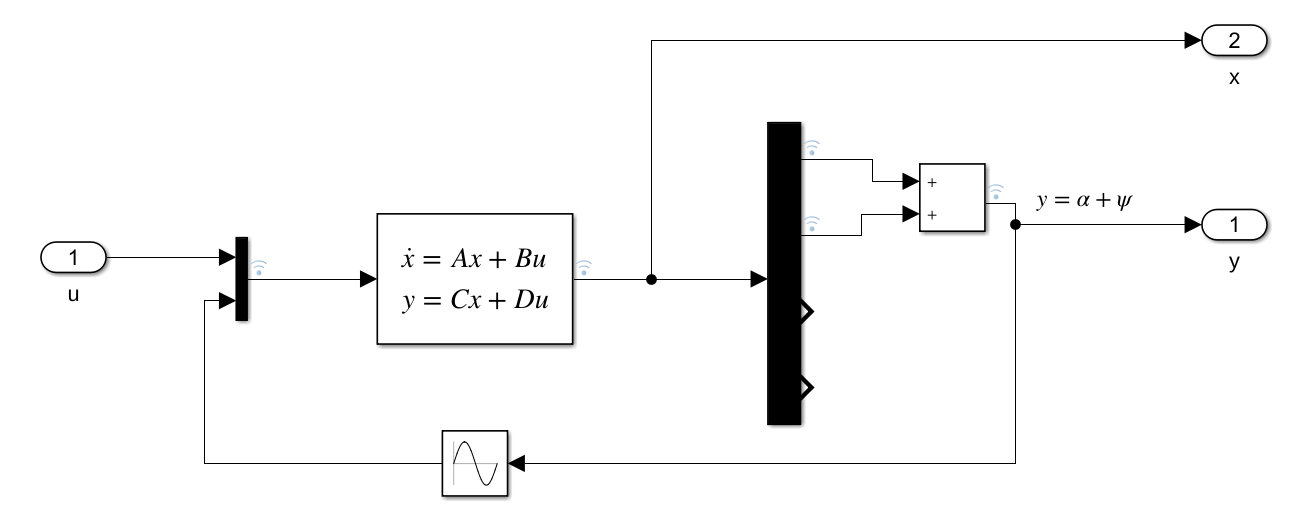
\includegraphics[width=0.7\textwidth]{modeleNL_schema.png}
  \caption{Modèle d'état simulé}
  \label{fig:label}
\end{figure}
En excitant le modèle avec un echelon on obtient :
\begin{figure}[ht]
  \centering
  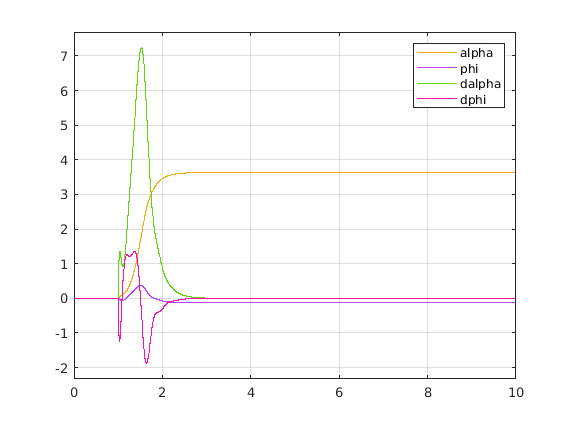
\includegraphics[width=0.7\textwidth]{modeleNL.png}
  \caption{Variable d'états en sortie du modèle}
  \label{fig:label}
\end{figure}
La simulation correspond au modèle attendu (on commande le systeme en position), il est stable mais non précis, de plus les dérivées sont assez chaotiques. 



\paragraph{Prépa.12}
À partir de la sortie $y$ il faut dérivé 4 fois pour que la commande $u$ apparaisse. on a donc
\begin{align*}
  z_1 & = y \\
  z_2 = \dot{z_1} &= \dot{x_1}+\dot{x_2} = x_3+ x_4 \\
  z_3 = \dot{z_2} &= \dot{x_3}+\dot{x_4} \\
      &= \frac{K_s}{J_b}x_2+\frac{mgh}{J_b}\sin(x_1+x_2)\\
  z_4 =  \dot{z_3} & = \frac{-K_s}{J_b}x_4+\frac{mgh}{J_b}(x_3+x_4)\cos(x_1+x_2)\\
  \dot{z_4} &= \frac{-K_s}{J_b}\left(
              -K_s\frac{(J_b+J_p)}{J_pJ_b}+ \frac{(N\phi)^2)}{RJ_p}x_3 - \frac{N\phi}{RJ_p}u +\frac{mgh}{J_b}\sin(x_1+x_2)
              \right)\\
              &+
              \frac{mgh}{J_b}\left(\frac{-K_s}{J_b}x_2+\frac{mgh}{J_b}\sin(x_1+x_2)
              \right)\cos(x_1+x_2) -
              \frac{mgh}{J_b}(x_3+x_4)^2\sin(x_1+x_2)
\end{align*}

On pose donc $v = \dot{z_4}$. 

\paragraph{Prépa.13}
On a fais les calculs en Prépa.13 , on peux donc réaliser le schéma bloc suivant :

\begin{figure}[H]
  \centering
  \begin{tikzpicture}
    \begin{scope}[at={(0,0)}]
    \node[draw, minimum height=1cm] (C) at (0,0) {
      \begin{tabular}[c]{c}
Synthèse \\de la commande
      \end{tabular}
};
    \node[draw, minimum height=1cm] (S) at (3.5,0) {$\dot{x}=f(x)+g(x)u$};
    \node[draw, minimum height=1cm] (N) at (7,0) {$z=\Phi(x)$};
    \draw[-latex] (-2,0) -- (C.west) node[near start,above]{$v$};
    \draw[-latex] (C.east) -- (S.west) node[near start, above]{$u$};
    \draw[-latex] (S.east) -- (N.west);
    \draw[-latex] (N.east) --  ++(1,0) node[above left]{$y$};
    \draw[-latex] (N.south) |- ++(-2,-1) node[near start,right]{$x$} -| (C.south);
  \end{scope}
  \node at (3,-2.5){\Large$\Updownarrow$};
  \begin{scope}[shift={(0,-4)}]
    \node[draw, minimum height=1cm] (I1) at (0,0) {$\int$};
    \node[draw, minimum height=1cm] (I2) at (2,0) {$\int$};
    \node[draw, minimum height=1cm] (I3) at (5,0) {$\int$};
\draw[-latex] (-2,0) -- (I1.west) node[near start, above]{$v$};
\draw[-latex] (I1.east) -- (I2.west) node[near start, above]{$z_n$};
\draw[-latex] (I2.east) -- ++(1,0) node[midway,above]{$z_{n-1}$};
\draw[-latex,dashed] (I2.east)++(1,0) -- (I3.west) node[near end, above]{$z_{2}$};
\draw[-latex] (I3.east) -- ++(2,0) node[near end, above]{$z_1=y$};
  \end{scope}
  \end{tikzpicture}
  \caption{Forme normale}
\end{figure}


\paragraph{Manip.2}
Pour réaliser le bouclage linéarisant, on utilise le fichier transmis au cours de TP au groupe (mon implémentation ne donnait pas de résultat attendu malgré les nombreux réglages effectués).

\begin{figure}[ht]
  \centering
  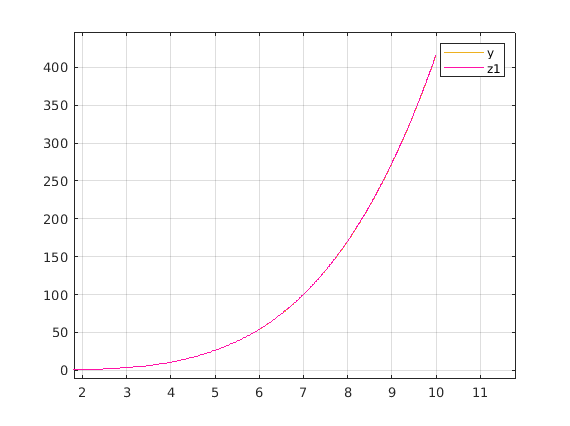
\includegraphics[width=0.7\textwidth]{BLin.png}
  \caption{Sortie du modèle et du bouclage}
  \label{fig:label}
\end{figure}
Les sorties issues du modèle non linéaire et du changement de variable sot identique, on a bien $y=z_1$.

\paragraph{Conclusion}

Dans ce TP on a mis en place une modélisation non linéaire d'un
système et utiliser une bouclage linéarisant pour pouvoir construire
un asservissement précis et rapide. Par manque de temps je n'ai pas pu
mettre en place la dernière partie concernant la planification de
trajectoire, qui sera par ailleurs étudié dans le TP2.

\end{document}

%%% Local Variables:
%%% mode: latex
%%% TeX-master: t
%%% End:
